
\section{Measurements}
\label{sec:meas}

\begin{figure}[t]
  \centering
  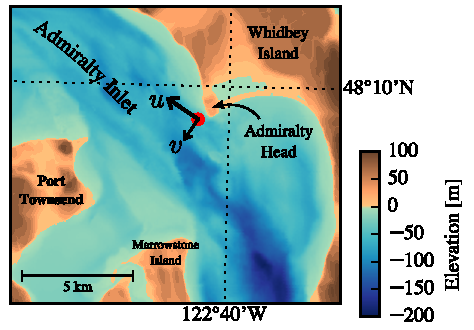
\includegraphics[width=3.4in]{map04_annot.pdf}
  \caption{Bathymetry of Admiralty Inlet near Port Townsend, Washington, U.S.A. \cite[]{Finlayson2005}. The red dot indicates the location of all measurements. The positive $u$ direction is the direction of ebb flow (thick arrow originating from red dot), and positive $v$ is away from Admiralty Head (smaller arrow).}
  \label{fig:map}
\end{figure}

This work focuses on measuring turbulence from ADVs that are equipped with IMUs and deployed from moving (moored) platforms.
%IMU's---also known as MARG (magnetic, angular-rate, gravity), or AHRS (attitude heading reference system) sensors---measure three axes of the Earth's magnetic field, angular rotation, and linear acceleration.\footnote{Within the inertial sensor literature, IMU is generally reserved for a MARG sensor without a magnetometer, but herein we refer to the entire group of sensors that measure motion using accelerometers and angular-rate sensors as IMUs.} These signals are then integrated using Kalman filters to estimate the orientation and motion of the sensor \cite[]{Barshan+Whyte1995, Marins++2001, Bachmann++2003}.
The ADVs utilized for these measurements were Nortek Vector ADVs equipped with Microstrain 3DM-GX3-25 IMU sensors. These IMUs captured all six components of the ADV motion (three components of angular rotation and three components of linear acceleration), as well as the orientation of the ADV pressure case. The sampling of the motion sensor is tightly synchronized with the ADV measurements. The IMU measures its motion at 1 kHz and uses internal signal integration (Kalman filtering) to output the motion signals at the same sample rate as the ADV's velocity measurements. This reduces aliasing of the IMU's motion measurements above the ADV's sample rate \cite[]{3DM-GX3_coning_sculling}. Cable-head ADVs were used throughout this work to allow for flexibility in the positioning of the ADV head relative to its pressure case.

All measurements used in this work were made in Admiralty Inlet, Washington, approximately 500 m west southwest of Admiralty Head in 60-m of water near 48\deg\ 9.18' N, 122\deg\ 41.22' W (Figure \ref{fig:map}). The site is approximately 6 km east of Port Townsend, and 1 km north of the Port Townsend to Coupeville ferry route.  Admiralty inlet is the largest waterway connecting Puget Sound to the Strait of Juan de Fuca, and it possesses a large semidiurnal tidal flow \cite[]{Thomson++2012, Polagye+Thomson2013}.  This work utilizes data from three distinct deployment platforms: the tidal turbulence mooring, a StableMoor buoy, and a simple sounding weight.  All data used in this analysis is available from the MHK data repository (http://mhkdr.openei.org; submission ids: 49, 50 and 51). Each of these platforms are briefly described below, and additional details, photos, and schematic diagrams can be found in Part 1.

\subsection{Tidal Turbulence Mooring}

The tidal turbulence mooring (TTM) is a simple mooring system with a strongback fin suspended between a steel clump-weight anchor weighing 1,200 kg when dry and a 0.93-m-diameter spherical steel buoy with a buoyancy of 320 kg. The ADV pressure cases were clamped to one side of the strongback fin and the ADV sensor head was positioned 10 cm in front of the fin's leading edge (Figure \ref{fig:ttm:diagram}). The leading edge of the fin is fastened inline with the mooring line. This configuration was designed to work like a weather vane, such that the drag on the fin held the ADV head upstream of the mooring components.  This work utilizes data from two TTM deployments. 

\subsubsection{June 2012 TTM deployment}

The first TTM deployment was in June 2012 from 17:30 on the 12th until 14:30 on the 14th (local; i.e., Pacific Daylight Time). Two Nortek ADVs were clamped to either side of the fin so that the axis of their cylindrical pressure cases were parallel with the leading edge of the strongback. The ADV heads were spaced 0.5 m apart vertically along the fin. Only one of these ADVs was equipped with an integrated IMU. This TTM also had an upward-looking acoustic Doppler profiler mounted on the mooring anchor.

Periods of time during which this mooring interfered with a beam of the Doppler profiler were identified by inspecting the profiler's acoustic amplitude signal. Periods during which one beam of the profiler had $>5\%$ higher acoustic amplitude than the other beams were flagged as ``contaminated" and excluded from averaging.  Five-minute averages in which more than 50\% of the data were contaminated in this way were masked as invalid.

\subsubsection{June 2014 TTM deployment}

The second TTM deployment was in 2014 from 06:00 on June 17 to 05:00 on June 19 (local time).  Two Nortek ADV-IMUs were mounted on this TTM, with their heads spaced 0.5 m apart along the fin. In this case, the pressure cases and ADV heads were inclined at an angle of 18$^\circ$ to the leading edge of the fin to account for mooring blowdown during strong currents (Figure \ref{fig:ttm:photo}). This change was made to reduce vibrational motion observed during the June 2012 deployment that was believed to be associated with the orientation of the pressure cases.

\begin{figure}[t]
  \centering
  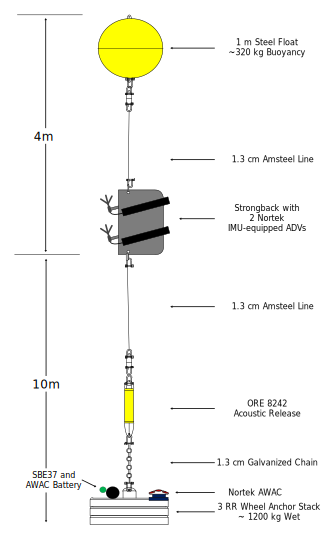
\includegraphics[width=2.4in]{TTM04b}
  \caption{Schematic diagram of the TTM; not to scale.}
  \label{fig:ttm:diagram}
\end{figure}

\begin{figure}[t]
  \centering
  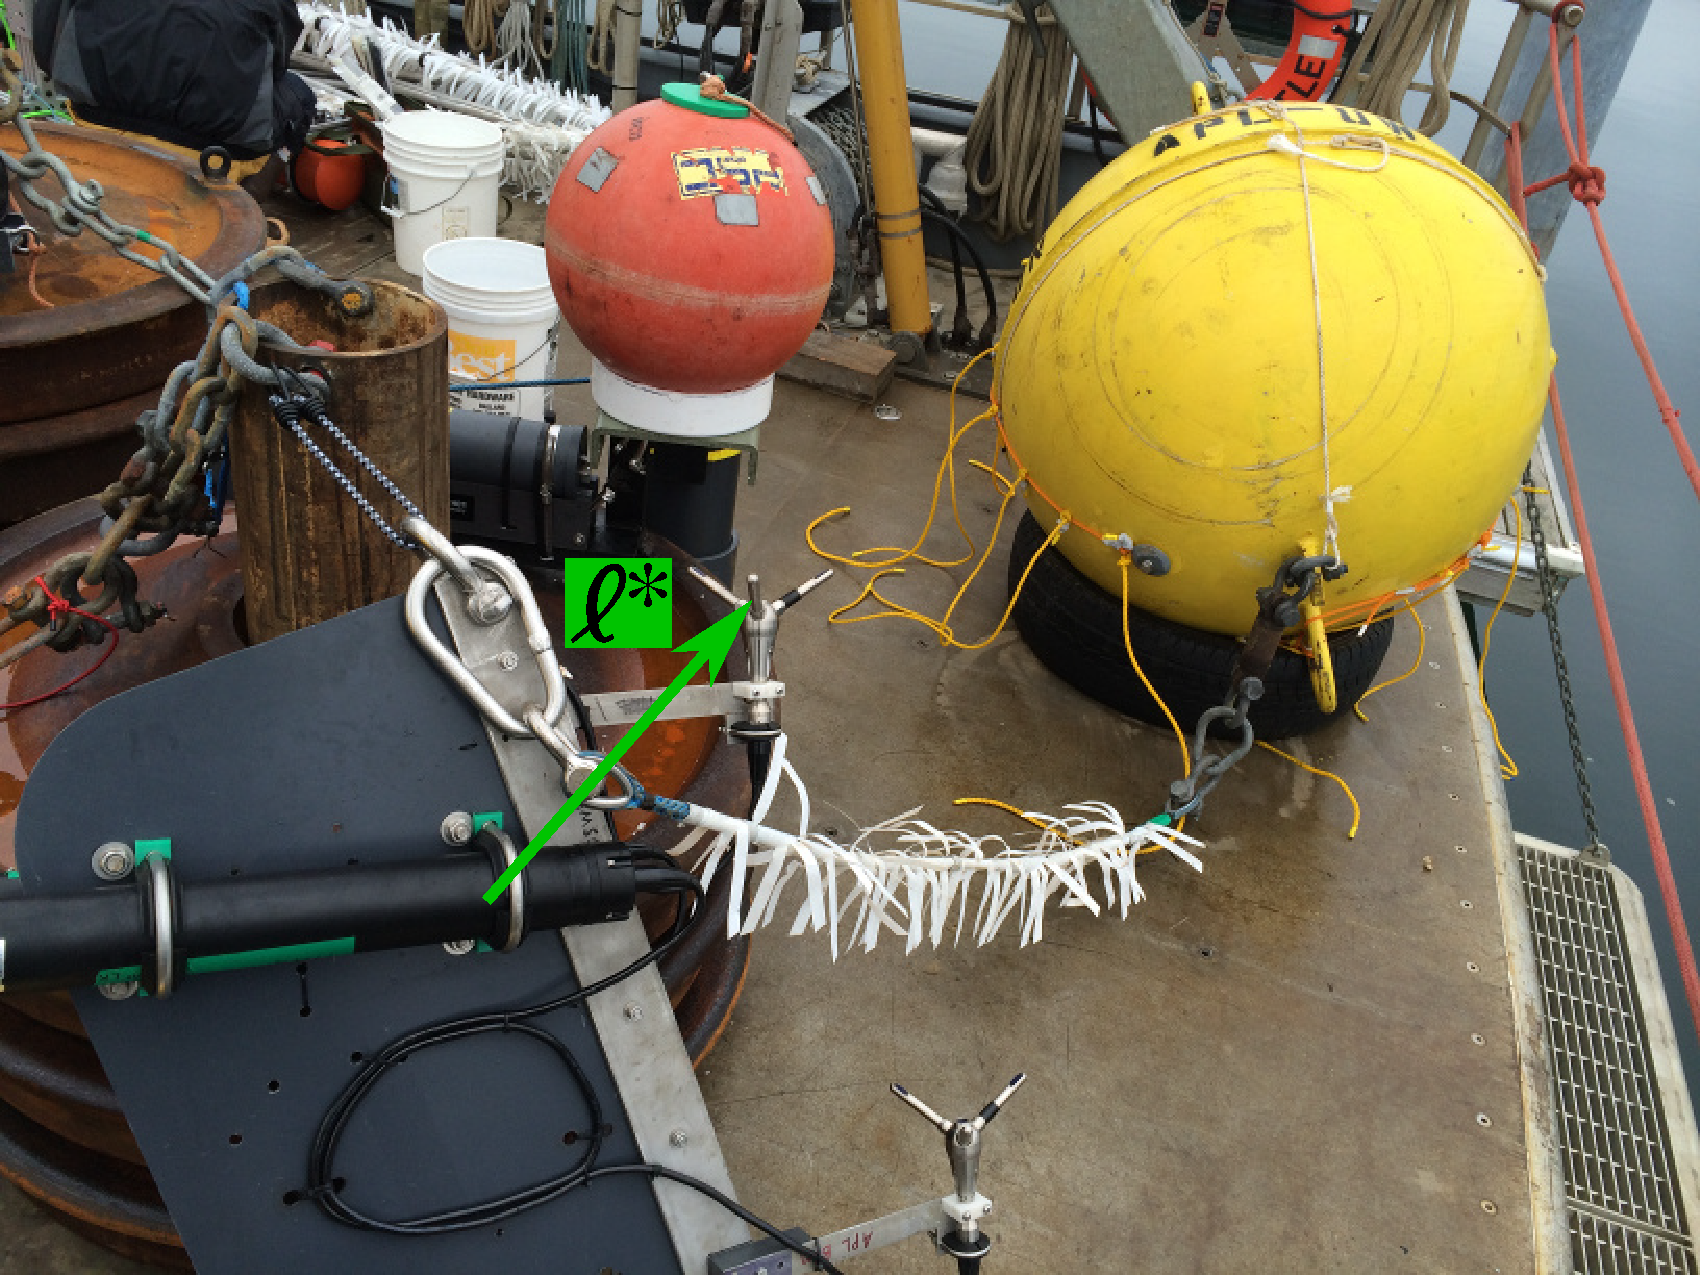
\includegraphics[width=2.6in]{TTM_image01_annot}
  \caption{TTM components on the deck of the R/V Jack Robertson. The TTM includes two ADVs, with pressure cases mounted on opposite sides of the fin. The anchor stack includes a pop-up buoy for retrieval. The green arrow indicates the vector from the IMU to the ADV head (face of the transmit transducer). }
  \label{fig:ttm:photo}
\end{figure}

\subsection{The StableMoor platform}

The second deployment platform was a cylindrical, StableMoor, syntactic foam buoy (manufacturer: Deep Water Buoyancy) that was anchored to a clump weight that weighed 2,700 lbs (Figure \ref{fig:SM}). The buoy is 3.5 m long and 0.45 m in diameter with a tail ring that is 0.76 m in diameter. The StableMoor buoy weighs 295 kg in air, and has a buoyancy of 185 kg in water. 

The StableMoor buoy was deployed with an ADV-IMU mounted at its nose from 11:21 on May 12 to 11:53 on May 13, 2015 (local time). The sample volume of the ADV is 10 cm forward of the nose and 20 cm above the center line of the StableMoor buoy (Figure \ref{fig:SM}). Based on \citeauthor{Wyngaard++1985}'s (1985) investigation of a similarly shaped slender body, the velocity measurements should have flow-distortion effects of less than 10\%. This configuration was designed to be the most stable platform for measuring turbulence from a moving platform. The StableMoor buoy was equipped with a 1,200-kHz RDI workhorse sentinel acoustic Doppler profiler that was oriented downward-looking to measure water velocity below the platform in twelve 1-m bins and measure buoy motion (``bottom tracking"), all at a 1-Hz sample rate. 

The buoy was ballasted to pitch upward a few degrees in zero-flow to avoid ``flying downward." In the presence of an oncoming current, the tail fins help to orient it into the flow. The anchor for this buoy is similar to that of the TTM, including an acoustic release so the mooring and anchor can be recovered separately.

The StableMoor platform has two primary advantages compared to the TTM. First, it is significantly more massive and hydrodynamically stable than the TTM, which reduces the frequency of motions of the platform. Second, the StableMoor platform is capable of supporting a bottom-tracking acoustic Doppler profiler, which provides an independent measure of the platform's translational motion. Disadvantages of the StableMoor include: its size, which adds to the challenge of deployment and recovery, and its cost, which is significantly higher than the TTM system.

\begin{figure}[t]
  \centering
  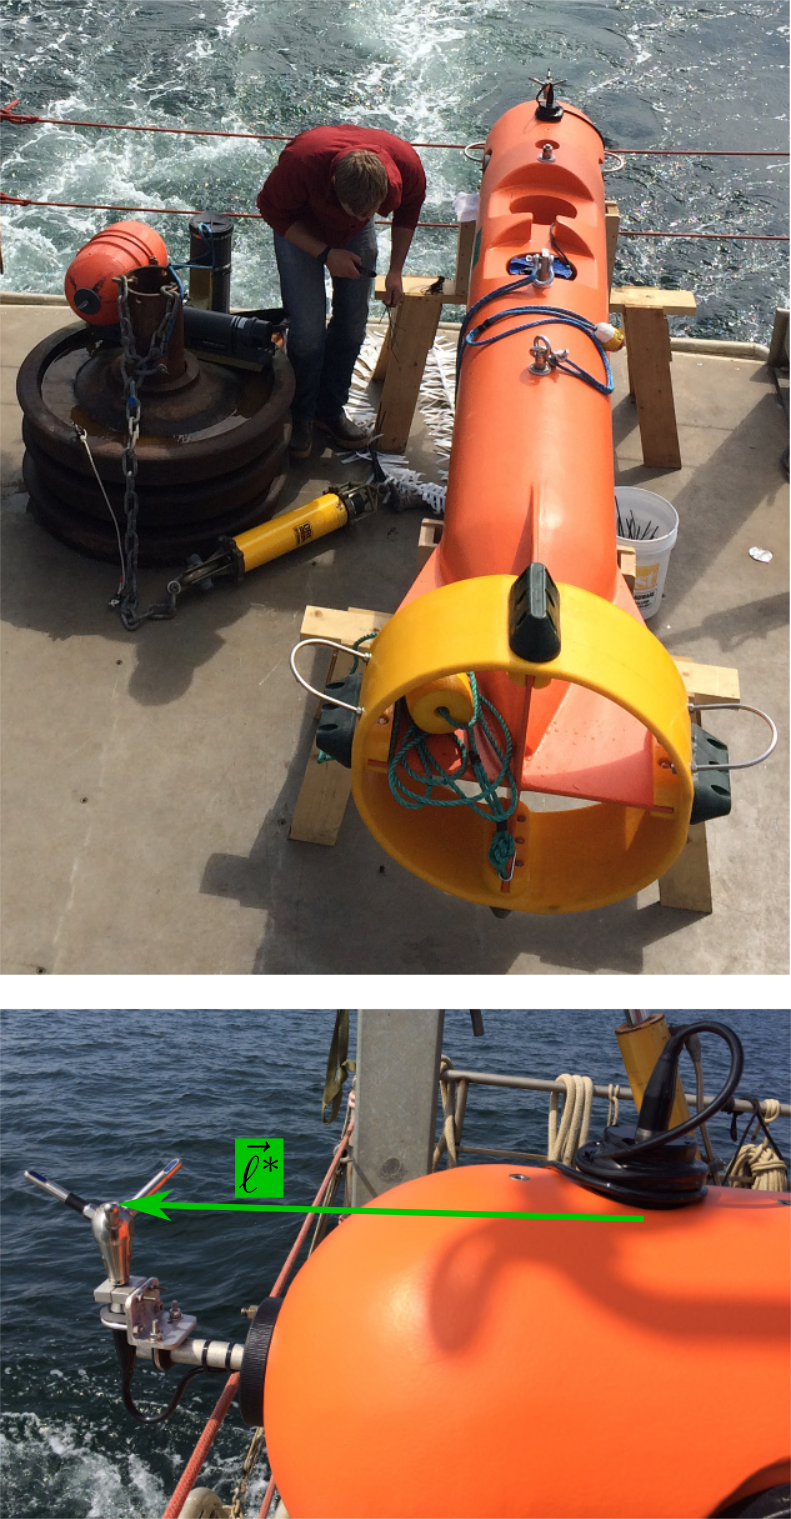
\includegraphics[width=2.6in]{StableMoor_Composite}
  \caption{Top: Alex DeKlerk checks to ensure that the StableMoor buoy is properly fastened to its anchor; the RDI workhorse ADCP can be seen in the rear instrument bay. A bridle is draped across the top of the buoy for deployment and recovery, and a small marker buoy fastened to the tail is useful during recovery.  Bottom: a close-up of the StableMoor with the ADV head and the top of its pressure case. The green arrow indicates the vector from the IMU to the ADV head. 
%Bottom: the StableMoor buoy in `wing mode', floating on the ocean surface with the marker buoy trailing behind. The ADV heads mounted at the ends of the cross-beam are protruding above the waterline.   
}
  \label{fig:SM}
\end{figure}

\subsection{Turbulence Torpedo}

The turbulence torpedo is a simple sounding weight with an ADV head mounted forward of the nose, and the ADV pressure case strapped below. This platform was deployed on May 14, 2015, for 37 minutes starting at 07:41 local time.  This measurement was made from a davit that hung the system from the side of the ship to a depth of approximately 25 m. The primary logistical advantages of this platform are its compact size, low cost, and the flexibility to perform spatial transects.  

\begin{figure}[th]
  \centering
  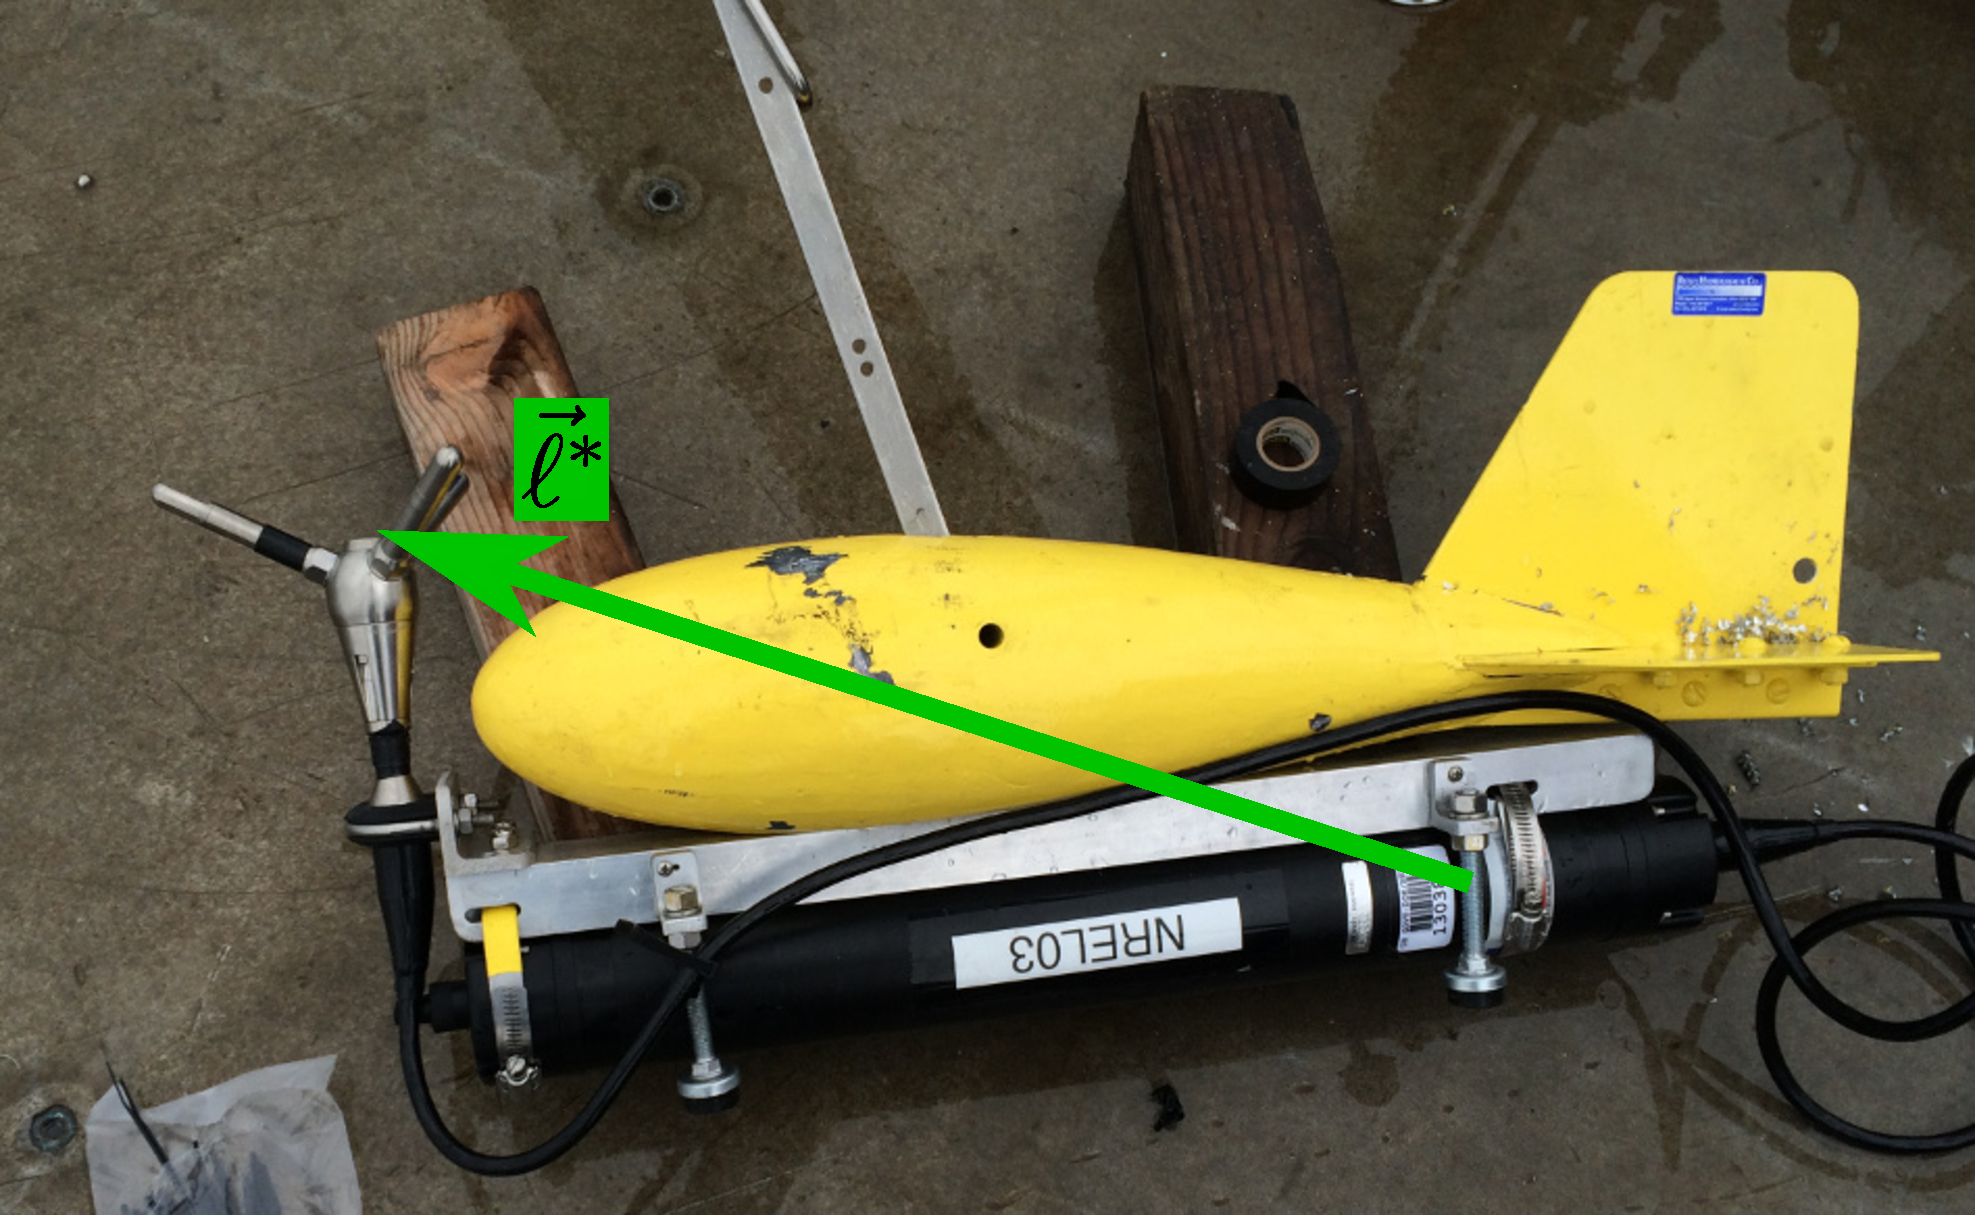
\includegraphics[width=2.6in]{Torpedo_Image01_annot}
  \caption{The turbulence platform showing details of the ADV head and pressure case configuration. The green arrow indicates the vector from the IMU to the ADV head. The head cable was taped out of the way beneath the sounding weight tail fins shortly after taking this photo.}
  \label{fig:torpedo}
\end{figure}

\subsection{Coordinate system and turbulence averaging}

Unless stated otherwise, vector quantities in this work are in a fixed ``principal-axes" coordinate system that is aligned with the bidirectional tidal flow: positive $u$ is in the direction of ebb (310$^\circ$ True), positive $w$ is vertically upward, and $v$ is the cross-stream component in a right-handed coordinate system. The full velocity vector, $\vec{\tilde{u}} = (\tilde{u}, \tilde{v}, \tilde{w})$, is separated into a mean and turbulent component as $\vec{\tilde{u}} = \vec{\bar{u}} + \vec{u}$, where the over-bar denotes a 5-minute average. Turbulence kinetic energy, $\tke = \uu + \vv+\ww$, and Reynold's stresses, $\uv$, $\uw$, $\vw$, are computed by averaging over the 5-minute window.  Throughout this work, we use $\bar{U} = (\bar{u}^2+\bar{v}^2)^{1/2}$ to denote the mean horizontal velocity magnitude. 

All spectra, $\spec{x}(f)=|\fourier{x(t)}|^2$, and cross spectra, $\cspec{x}{y}(f)=\mathrm{real}(\fourier{x(t)}\fourier{y(t)})$, are computed using NumPy fast Fourier transform routines \cite[]{Walt++2011}. Here, $\fourier{x(t)}$ denotes the fast Fourier transform of a signal $x(t)$. Time series, e.g., $x(t)$, are linearly detrended and Hanning windowed prior to computing $\fourier{x}$ to reduce spectral reddening.  

Throughout the remainder of this work, the dependence of $S$ and $C$ on $f$ is implied (e.g., $\spec{x}(f)$ is hereafter $\spec{x}$), and for other variables the dependence on $t$ is implied. Spectra and cross spectra are normalized to preserve variance: $\int \spec{u}\mathrm{d}f = \uu$, and  $\int \cspec{u}{v}\mathrm{d}f = \uv$. The notations $\spec{\ue}=(\spec{u}, \spec{v}, \spec{w})$, and $C\{\ue\} = (\cspec{u}{v}, \cspec{u}{w}, \cspec{v}{w} )$ denote the set of spectra and cross spectra for each velocity component and pairs of components, respectively.

Turbulence dissipation rates are computed as:
\begin{align}
  \epsilon = \frac{1}{\bar{U}}\left(\alpha\left\langle(\spec{u}+\spec{v}+\spec{w})f^{5/3}\right\rangle_{f_{IS}}\right)^{3/2}
\end{align}
Where  $\alpha=0.5$, and $\langle\rangle_{f_{IS}}$ denotes an average over the inertial subrange of the velocity spectra and where the signal-to-noise ratio is small \cite[]{Lumley+Terray1983,Sreenivasan1995}. Throughout this work, we take this average from 0.3 to 1 Hz for the $u$ and $v$ components, and 0.3 to 3 Hz for the $w$ component.

%%% Local Variables:
%%% mode: latex
%%% TeX-master: "Kilcher_etal_IMU-ADV"
%%% End:
